\documentclass{article}
\usepackage[utf8]{inputenc}
\usepackage{amsmath}
\usepackage{amsthm}
\usepackage{amssymb}
\usepackage{mathtools}
\usepackage{stmaryrd}
\usepackage[english]{babel}
\newtheorem{theorem}{Theorem}
\newtheorem{definition}{Definition}
\newtheorem{lemma}{Lemma}
\usepackage[margin=1.0in]{geometry}

\title{COMP330 Notes}
\author{Chany Ahn}
\date{September 2021 - December 2021}

\begin{document}

\maketitle
\newpage
\tableofcontents
\newpage
\section{Logic}
\subsection{Equivalence Relations}
A binary relation $R$ on a set $X$ is a subset of $X \times X$. Notation: $(a,b) \in \mathbb{R}$ or $aRb$. $R$ must satisfy:
\begin{enumerate}
    \item Reflexivity: $\forall x \in X, xRx$.
    \item Symmetry: $\forall x,y \in X, xRy \Rightarrow yRx$.
    \item Transitivity: $\forall x,y,z \in X, xRy, yRz \Rightarrow xRz$.
\end{enumerate}

\subsection{Partial Order}
This is an abstraction of $\leq$. A binary relation $R$ is a partial order of $X$ if:
\begin{enumerate}
    \item $\forall x \in X, xRx$.
    \item $\forall x,y \in X, xRy, yRx \Rightarrow x = y$ (Antisymmetry).
    \item $\forall x,y,z \in X, xRy, yRz \Rightarrow xRz$.
\end{enumerate}
If every pair of elements can be compared, then we have a \textit{total order} (aka \textit{linear order}).
\subsection{Well-Founded Orders}
A parital order $\leq$ on $S$ is well founded if every non-empty subset $U \subseteq S$ has a \underline{minimal element}. We say $u \in U$ is minimal if there is nothing else in $U$ strictly less than $u$.

\begin{theorem}
The principle of induction can be used if and only if the order is well-founded.
\end{theorem}
\section{Deterministic Finite Automata}
\begin{definition}
Some useful definitions:
\begin{itemize}
    \item $\Sigma$: A set of letters (or an alphabet).
    \item $\Sigma^*$: Set of all words that can be made by the alphabet $\Sigma$.
    \item $L \subseteq \Sigma^*$: A language.
\end{itemize}
\end{definition}
\begin{definition}
A deterministic finite automaton (DFA) is a 4-tuple:
\begin{itemize}
    \item $S$: A finite set of states.
    \item $s_0 \in S$: The start state.
    \item $\delta : S\times \Sigma \rightarrow S$: Transition function.
    \item $F \subseteq S$: Accepting states.
\end{itemize}
\end{definition}
\begin{definition}
A languages that is recognized by a DFA is called a regular language.
\end{definition}
\noindent\textit{Understand the examples from class!}
\section{Nondeterministic Finite Automata}
\begin{definition}
A nondeterministic finite automata is a 4-tuple:
\begin{itemize}
    \item $Q$: A finite set of states.
    \item $Q_0 \subseteq Q$: A set of start states ($Q_0 \ne \varnothing$).
    \item $F \subseteq Q$: A set of accepting states.
    \item $\Delta$: A transition relation.
    \begin{itemize}
        \item $\Delta : Q \times \Sigma \rightarrow \mathcal{P}(Q)$
        \item $\Delta(q, a)$: all the places the machine can go to if it is in $q$ and reads an $a$.
    \end{itemize}
\end{itemize}
\end{definition}
\begin{definition}
An NFA with $\varepsilon$-moves is a machine that can jump to a new state without reading a letter.
\end{definition}
\begin{theorem}
The language accepted by an NFA is a regular language.
\end{theorem}
\begin{definition}
\begin{align}
    \delta^* &: S \times \Sigma^* \rightarrow S\\
    \Delta^* &: \mathcal{P}(Q) \times \Sigma^* \rightarrow \mathcal{P}(Q)
\end{align}
\end{definition}
\noindent These equalities follow from the above definition for (1) which is defined inductively for $a \in \Sigma$ and $w \in \Sigma^*$.
\begin{align*}
    \delta^*(s,\varepsilon) &= \varepsilon\\
    \delta^*(s,wa) &= \delta(\delta^*(s,w), a)\\
    \delta^*(s,aw) &= \delta^*(\delta(s,a), w)
\end{align*}
Similary, we have for (2), given $A \subseteq Q$:
\begin{align*}
    \Delta^*(A, \varepsilon) &= A\\
    \Delta^*(A, wa) &= \bigcup_{q \in \Delta^*(A,w)}\Delta(q,a)
\end{align*}
\noindent\textbf{Facts}:
\begin{itemize}
    \item $\delta^* (s, xy) = \delta^*(\delta^*(s,x),y)$
    \item $\Delta^*(A \cup B,w) = \Delta^*(A,w) \cup \Delta^*(B,w)$
    \item $\Delta^*(A,xy) = \Delta^*(\Delta^*(A,x), y)$
\end{itemize}
\begin{definition}
Given a DFA, $M = (S,s_0,\delta,F)$, $L(M) = \{w \in \Sigma^* | \delta^*(s_0,w) \in F\}$.
\end{definition}
\begin{definition}
Given an NFA, $N = (Q,Q_0,\Delta,F)$, $L(N) = \{w \in \Sigma^* | \Delta(Q_0,w) \cap F \ne \varnothing\}$.
\end{definition}
\begin{theorem}
Given an NFA, $N$, there exists a DFA, $M$, s.t. $L(M) = L(N)$.
\end{theorem}
\begin{proof}
Let, $M = (S,s_0,\delta,F)$, $N = (Q,Q_0,\Delta,F)$, $S = \mathcal{P}(Q)$, $s_0 = Q_0$, $\hat{F} = \{A \subseteq Q | A \cap F \ne \varnothing\}$, $\delta(A,a) = \bigcup_{q \in A}\Delta(q,a) = \delta^*(A,a)$. We require the following lemma:
\begin{lemma}
$\Delta(A,w) = \delta^*(A,w)$ $\forall w \in \Sigma^*$.
\end{lemma}
\noindent The proof is as follows:
\begin{align*}
    L(N) &= \{w | \Delta^*(Q_0,w) \cap F \ne \varnothing\}\\
    &= \{w | \Delta^*(Q_0,w) \in \hat{F}\} \text{ (Defn of }\hat{F})\\
    &= \{w | \delta^*(Q_0,w) \in \hat{F}\}\\
    &= \{w | \delta^*(s_0,w) \in \hat{F}\} = L(M)
\end{align*}
\end{proof}
\section{Closure Properties of Regular Languages}
\begin{theorem}
The following operations preserve regularity: if $L_1, L_2$ are regular languages, then
\begin{enumerate}
    \item $L_1 \cup L_2$ is regular.
    \item $L_1 \cap L_2$ is regular.
    \item $L_1 \cdot L_2 = \{xy | x \in L_1, y\in L_2\}$.
    \item $\overline{L} = \{x \in \Sigma^* | x \notin L\}$.
    \item $L^* = \{x_1 \ldots x_n | \forall n \geq 0, x_i \in L\}$ ($\varepsilon$ is always in $L^*$ even if it is not in $L$).
\end{enumerate}
\end{theorem}
\begin{proof}
Let $M_1 = (S_1, s_0^{(1)}, \delta_1, F_1)$, $M_2 = (S_2, s_0^{(2)}, \delta_2, F_2)$, $L(M_1) = L_1$, $L(M_2) = L_2$.
\begin{enumerate}
    \item We construct an NFA, $N$:
    \begin{itemize}
        \item $Q = S_1 \cup S_2$ ($S_1 \cap S_2 \ne \varnothing$)
        \item $Q_0 = \{s_0^{(1)},s_1^{(2)}\}$
        \item $F = F_1 \cup F_2$
        \item $\Delta(s,a) = \begin{cases}
        \{\delta_1(s,a)\} &\text{if } s\in S_1\\
        \{\delta_2(s,a)\} &\text{if } s\in S_2
        \end{cases}$
    \end{itemize}
    \item In this case we construct a DFA
    \begin{itemize}
        \item $S = S_1 \times S_2$
        \item $s_0 = (s_0^{(1)},s_1^{(2)}) \in S_1 \times S_2$
        \item $\delta((s_1,s_2), a) = (\delta_1(s_1,a),\delta_2(s_2,a))$
        \item $F = F_1 \times F_2$
    \end{itemize}
    \item Construct NFA, $N = (Q, Q_0, \Delta, F)$:
    \begin{itemize}
        \item $Q = S_1 \cup S_2$ $(S_1 \cap S_2 = \varnothing)$
        \item $Q_0 = \{s_0^{(1)}\}$
        \item $\Delta(s,a) = \begin{cases}
        \{\delta_1(s,a)\} &\text{if } s\in S_1\\
        \{\delta_2(s,a)\} &\text{if } s\in S_2
        \end{cases}$
        \item $\Delta(t, \varepsilon) = \{s_0^{(2)}\}$ $t\in F_1$
        \item $F = F_2$
    \end{itemize}
    \item Exercise
    \item (Watch this part of the lecture) Let $M = (S, s_0, \delta, F)$, $L(M) = L$. We construct the NFA, $N = (Q, Q_0, \Delta, F)$:
    \begin{itemize}
        \item $Q = S \cup \{q_0\}$ where $q_0$ is a new state
        \item $Q_0 = \{q_0\}$
        \item $\hat{F} = F \cup \{q_0\}$
        \item $\Delta(q,a) = 
        \begin{cases} 
        \{\delta_1(q,a)\} & \text{if } q \in S \text{ \& } a \ne \varepsilon, q \notin F\\
        \{\delta_1(q,a)\} & \text{if } q \in F \text{ \& } a \ne \varepsilon\\
        \{s_0\} & \text{if } q \in F  \text{ \& } a = \varepsilon\\
        \{s_0\} & \text{if } q = q_0 \text{ \& } a = \varepsilon
        \end{cases}$
    \end{itemize}
    This machine accepts exactly the words in $L^*$. Argue that any word accepted must be in $L^*$.
\end{enumerate}
\end{proof}
\noindent\textit{See class examples!}
\subsection{Regular and Non-Regular Languages}
The purpose of this section is to keep track of the languages seen in class that are regular or not (can be useful for counter-examples).
\subsubsection{Regular Languages}
\subsubsection{Non-Regular Languages}
\section{Algebra of Regular Expressions}
\begin{definition}
Fix an alphabet $\Sigma$. The collection of regular expressions over $\Sigma$, $(Reg(\Sigma))$, is defined by induction as follows:
\begin{enumerate}
    \item $\varnothing$ is a regular expression.
    \item $\varepsilon$ is a regular expression.
    \item If $a \in \Sigma$, then $a$ is a regular expression.
    \item If $R_1,R_2$ are regular expressions, then so is $R_1 + R_2$.
    \item If $R_1, R_2$ are regular expressions, the so is $R_1R_2$.
    \item If $R$ is a regular expression, so is $R^*$.
\end{enumerate}
$\llbracket R \rrbracket$ is the set denoted by $R$.
\begin{itemize}
    \item $\llbracket \varnothing \rrbracket = \varnothing$
    \item $\llbracket \varepsilon \rrbracket = \{\varepsilon\}$
    \item $\llbracket R_1 + R_2 \rrbracket = \llbracket R_1 \rrbracket \cup \llbracket R_2 \rrbracket$
    \item $\llbracket R_1R_2 \rrbracket = \llbracket R_1 \rrbracket\llbracket R_2 \rrbracket = \{xy | x \in \llbracket R_1 \rrbracket, y\in \llbracket R_2 \rrbracket\}$
    \item $\llbracket R^* \rrbracket = \bigcup_{i=0}^{\infty}\llbracket R \rrbracket \ldots \llbracket R \rrbracket$
\end{itemize}
\end{definition}
\begin{theorem}
(Kleene's Theorem)
A language is regular if and only if it is defined by a regular expression.
\end{theorem}
\begin{proof}
Lol this thing is so long. Do later.
\end{proof}
\subsection{Kleene Algebra}
Regular expression form an algebra. It has two binary operations $+, \cdot$, one unary operation $*$, and 2 constants $\varnothing, \varepsilon$. The basic equations are as follows (more can be derived):
\begin{enumerate}
    \item $R+\varnothing = \varnothing + R = R$
    \item $R+S = S+R$
    \item $R + (S+T) = (R+S) +T$
    \item $R+R = R$
    \item $R\cdot\varnothing = \varnothing \cdot R = \varnothing$
    \item $R\cdot\varepsilon = \varepsilon \cdot R = R$
    \item $R\cdot(S \cdot T) = (R \cdot S) \cdot T$
    \item $R \cdot (S + T) = R \cdot S + R \cdot T$
    \item $(R+S) \cdot T = R \cdot T + S \cdot T$
    \item $\varepsilon + RR^* = \varepsilon + R^*R = R^*$
\end{enumerate}
Other equations include: $(R^*)^* = R^*$, $(R^*S)^*R^* = (R+S)^*$.
\section{Pumping Lemma}
\begin{definition}
(Informal) The pumping lemma is an essential property of regular languages. It says that all sufficiently long strings in a regular language may be pumped -- that is, have a middle section of the string repeated an arbitrary number of times -- to produce a new string that is also a part of the language.
\end{definition}
\begin{definition}
\underline{Pigeon-Hole Principle}: If you have $n$ boxes and $m$ objects where $m > n$, if you put all the objects into theses boxes, at least one box will have more than one object.
\end{definition}
\begin{lemma}
The Pumping Lemma\\
If L is a regular language, $\exists p \in \mathbb{N}\ p > 0$ s.t. $\forall w \in L\ |w| \geq p\ \exists x,y,z \in \Sigma^*$ s.t.:
\begin{enumerate}
    \item $w = xyz$
    \item $|xy| \leq p$
    \item $|y| > 0$
\end{enumerate}
$\forall i \in \mathbb{N}$, $xy^iz \in L$.
\end{lemma}
\noindent So, $L$ is regular $\Rightarrow L$ can be pumped. The contrapositive is: $L$ cannot be pumped $\Rightarrow L$ is not regular. The contrapositive is how the pumping lemma is used.

\noindent The above statements formally:
\begin{align*}
    L \text{ regular} \Rightarrow &[\exists p > 0 \forall s \in L\ |s| \geq p \Rightarrow \exists x,y,z \in \Sigma^*\\ &(s = xyz \land |xy| \leq p \land |y| > 0 \land \forall i \geq 0, xy^iz \in L)] \Rightarrow L \text{ can be pumped.}\\
\end{align*}
\underline{Note}: Negating quantified statements.
\begin{itemize}
    \item $\neg(\forall x\ \varphi(x)) \equiv \exists x\ \neg\varphi(x)$
    \item $\neg(\exists x\ \varphi(x)) \equiv \forall x\ \neg\varphi(x)$
\end{itemize}
\begin{align*}
    &L \text{ cannot be pumped.} \Rightarrow \neg [\cdot]\\ &\Rightarrow
    [\forall p, p > 0 \Rightarrow \exists w \in L \land |w| \geq p \land \forall x,y,z \in \Sigma^*\\ &(w = xyz \land |xy| \leq p \land |y| > 0) \Rightarrow \exists i\ xy^iz \notin L] \Rightarrow L \text{ not regular.}
\end{align*}
\underline{Note}: A universally quantified statement on an empty set is always true.
\subsection{Examples}
\begin{enumerate}
    \item $L = \{a^nb^n | n \geq 0\}$\\
    Demon chooses p, I choose $a^pb^p$.
    
    Demon has to break up $a^pb^p$ into 3 pieces: $xyz$.
    
    Assume $|xy| \leq p$, $|y| > 0$. The string looks like $aa\ldots abb \ldots b$. $y$ must be in the string of $a$'s, and $|y| \geq 1$. Choose $i=2$, in which case we can obtain $xyyz$.
    
    I have inserted at least one extra $a$, and I have not changed the $b$'s, so clearly the number of $a$'s and the number of $b$'s cannot be equal. Thus, $xyyz \notin L$. So, $L$ cannot be regular.
    \item $L = \{a^nb^ma^{n+m} | n,m > 0\}$
    
    Demon: $p$, Class: $a^pb^pa^{2p}$.
    
    Demon has to choose $xy$ to consist purely of $a$'s and $y$ cannot be empty ($|y| = l > 0$). The class chooses $i=2$. This gives $xy^2z = a^{p+l}b^pa^{2p}$, but $p+l+p \ne 2p$, so $xy^2z \notin L$.
    \item $L = \{ab^na^n | n > 0\}$
    
    Demon: $p$, Class $ab^pa^p$.
    
    The demon must consider some cases:
    \begin{enumerate}
        \item $x = \varepsilon$, $y = a$
        \item $x = a$, $y = b^l$ where $p \geq l > 0$
        \item $x = ab^m$, $y = b^l$ where $p \geq l > 0$
    \end{enumerate}
    The class must display that, after choosing $i=2$, $xy^2z \notin L$.
    \item Question: Supposed $L \subseteq \{a,b\}^*$, and suppose $L$ is infinite. If every word $w$ in $L$ satisfies $\#_a(w) = \#_b(w)$, is it possible that $L$ could be regular?
    
    A: YES!
    
    Consider $(ab)^*$. This is regular, is infinite, and every word has an equal number of $a$'s and $b$'s. Furthermore, it is easy to construct a DFA for this language.
    \item 
\end{enumerate}
\section{Minimization}
Sometimes, DFA's may have more states than are required (seeing as we can actually define a lower-bound for the number states for any given DFA). Thus, the point of this section is to define minimization techniques for a DFA to simplify our solution.
\begin{definition}
Given a DFA $M = (D, s_0, \delta, F)$ over alphabet $\Sigma$, we say $p,q \in S$ are \underline{equivalent} (and write $p \approx q$) if $\forall x \in \Sigma^*$, $\delta^*(p,x) \in F \iff \delta^*(q,x) \in F$.
\end{definition}

\noindent \underline{Remark}: $p \not\approx q$ means $\exists x \in \Sigma^*$, $\delta^*(p,x) \in F$ and $\delta^*(q,x) \not\in F$ or $\delta^*(p,x) \notin F$ and $\delta^*(q,x) \in F$. (Note that $\approx$ is an equivalence relation.)
\begin{lemma}
$p \approx q \Rightarrow \forall a \in \Sigma$, $\delta(p,a) \approx \delta(q,a)$.
\end{lemma}
\begin{proof}
Assume $p \approx q$. Suppose $\delta^*(\delta(p,a),x) \in F$, i.e. $\delta^*(p,ax) \in F$. Since we assumed $p \approx q$ then $\delta^*(q,ax) \in F$ and $\delta^*(\delta(q,a),x) \in F$. Similarly, in the reverse direction. Thus, $\delta(p,a) \approx \delta(q,a)$.\\
\end{proof}
\noindent Note on notation: $p \approx q$ means $[p] = [q]$, so the lemma can be restated as: $[p] = [q] \Rightarrow \forall a \in \Sigma$, $[\delta(p,a)] = [\delta(q,a)]$.

\noindent So the shrunken machine is defined as follows:
\begin{itemize}
    \item $S' =$ equivalence classes: $S/\approx$ (the collection of equivalence classes).
    \item $S_0' = [s_0]$.
    \item $\delta'([p],a) = [\delta(p,a)]$ (which is well-defined because of the lemma).
    \item $F' = \{[s] | s\in F\}$.
\end{itemize}
\begin{lemma}
$p \in F$ and $p \approx q \Rightarrow q \in F$. (Gotta think about this one)
\end{lemma}
\begin{lemma}
$\forall w \in \Sigma^*$, $\delta'^*([p],w) = [\delta^*(p,w)]$.
\end{lemma}
\begin{proof}
Induction on $w$.
\begin{itemize}
    \item Base case: $w = \varepsilon$.
    \[\delta'^*([p],\varepsilon) = [p] = [\delta^*(p,\varepsilon)]\]
    \item Inductive step: Assume $\delta'^*([p],w) = [\delta^*(p,w)] \leftarrow$ WTS $\forall a \in \Sigma$, $\delta'^*([p],wa) = [\delta^*(p,wa)]$.
    \begin{align*}
        \delta'^*([p],wa) &= \delta'(\delta'^*([p],w),a)\\
        &= \delta'([\delta^*(p,w)],a) \text{ Inductive Hypothesis}\\
        &= [\delta(\delta^*(p,w),a)] \text{ Def. of } \delta'\\
        &= [\delta^*(p,wa)] \text{ Def. of } \delta^*
    \end{align*}
\end{itemize}
\end{proof}
\begin{theorem}
$L(M') = L(M)$.
\end{theorem}
\begin{proof}
\begin{align*}
    x \in L(M') &\iff \delta'^*([s_0],x) \in F'\\
    &\iff [\delta^*(s_0,x)] \in F'\\
    &\iff \delta^*(s_0,x) \in F\\
    &\iff x \in L(M)
\end{align*}
\end{proof}
\subsection{Algorithm based on this $\approx$}
\underline{Idea}: Start by putting all the states into 2 groups: accept, reject. Keep splitting the groups.

\bigbreak\noindent \underline{Notation}: $p \bowtie q$ if $p \not\approx q$. i.e. $\exists w \in \Sigma^*$ s.t. $\delta^*(p,w) \in F$ and $\delta^*(q,w) \notin F$ or the other way around.

\bigbreak\noindent \underline{Fact}: If $\exists a \in \Sigma$ s.t. $\delta(p,a) \bowtie \delta(q,a)$, then $p \bowtie q$.

\bigbreak\noindent\underline{Algorithm}: Define an $S \times S$ array of booleans:
\begin{enumerate}
    \item For every pair $(p,q)$ s.t. $p \in F$ and $q \notin F$, we put a 0 in the $(p,q)$ cell.
    \item Repeat until no more changes:
    
    For each pair $(p,q)$ not marked 0, check if $\exists a \in \Sigma$ s.t. $(\delta(p,a), \delta(q,a))$ is marked 0. If yes put a 0 in $(p,q)$.
    \item Mark everything remaining with a 1.
\end{enumerate}
\begin{theorem}
If two states are not labelled 0 by the algorithm, they are equivalent.
\end{theorem}
\begin{proof}
Suppose the machine is $(S, s_0, \delta, F)$. Assume the theorem is false. There is a pair of states that are not equivalent but which the algorithm fails to mark. Call such a pair a BAD pair. Suppose 2 states are not equivalent, then there is a string that distinguishes them, i.e. $\exists x \in \Sigma^*$ s.t. $\delta^*(p,x) \in F$ and $\delta^*(q,x) \notin F$. Among all such bad pairs, choose the one with the shortest distinguishing string. Note, $\varepsilon$ cannot be such a distinguishing string.

Lets assume $(s,t)$ is a bad pair, and its distinguishing string $x = x_1x_2x_3\ldots x_n$ is the shortest one possible. Now consider $\delta(s,x_1)$ and $\delta(s,x_2)$. This pair is not equivalent since:
\[\delta^*(\delta(s,x_1,x_1\ldots x_n) \in F,\ \delta^*(\delta(t,x_1,x_1\ldots x_n) \notin F\]
so $\delta(s,x_1) \bowtie \delta(t,x_1)$. But it cannot be a bad pair because its distinguishing string is strictly smaller than $x$. So the algorithm must have marked $(\delta(s,x_1), \delta(t,x_1))$ with a 0 at some stage. But in the next step, it has to mark $(s,t)$ which is a contradiction. Thus, there are no bad points.\\
\end{proof}
\noindent\underline{Running Times}:
\begin{itemize}
    \item Basic algorithm: $O(n^4)$.
    \item Improved algorithm maintains a list of pairs that will be immediately distinguished if $s,t$ are distinguished: $O(n^2k)$ ($n^2$ comes from the states and $k$ is the size of the alphabet).
    \item Clever algorithm (John Hopcroft):  $O(n\log n)$ which is the best possible.
    \item Old algorithm: exponential time.
\end{itemize}
\section{Myhille-Nerode Theorem}
\begin{definition}
An equivalence relation, $R$, on $\Sigma^*$ is said to be right-invariant if $\forall x,y \in \Sigma^*$, $xRy \Rightarrow \forall z \in \Sigma^*$, $xzRyz$.
\end{definition}
\begin{itemize}
    \item \underline{Major example}: Given a DFA $M = (Q,\Sigma, q_0, \delta,F)$, where $\delta^* : Q \times \Sigma^* \rightarrow Q$: $\forall q \in Q$, $\delta^*(q,\varepsilon) = q$. $a \in \Sigma$, $x \in \Sigma^*$, $\delta^*(q,ax) = \delta^*(\delta(q,a),x)$, it follows $\delta^*(q,xy) = \delta^*(\delta^*(q,x),y)$. (Watch this part of the lecture)
\end{itemize}
\begin{definition}
We define $R_M$ based on $M$. $xR_My$ if and only if $\delta^*(q_0,x) = \delta^*(q_0,y)$.
\end{definition}
This is clearly an equivalence relation, and it is right invariant (prove if your bored).
\begin{definition}
Given any language $L \subseteq \Sigma^*$ (not necessarily regular), we define an equivalence relation as $\equiv_L$:
\[x \equiv_L y\ \text{iff}\ \forall z,\ xz \in L \iff yz \in L\]
\end{definition}
\begin{lemma}
$\equiv_L$ is right-invariant.
\end{lemma}
\begin{theorem}
(Myhill-Nerode) The following are equivalent:
\begin{enumerate}
    \item $L$ is accepted by a DFA i.e. $L$ is a regular language.
    \item $L$ is the union of some of the equivalence classes of some right-invariant equivalence relation of finite index.
    \item The equivalence relation $\equiv_L$ has a finite index.
\end{enumerate}
\end{theorem}
\begin{proof}
We will show $(1) \Rightarrow (2) \Rightarrow (3) \Rightarrow (1)$.
\begin{itemize}
    \item $(1) \Rightarrow (2)$: We assume $L$ is recognized by a DFA, $M=(Q,\Sigma, q_0,\delta,F)$. We've already seen that $R_M$ defined above is right-invariant. Thus, $R_m$ has, at most, $|Q|$ equivalence classes, thus $R_m$ definitely has a finite index. The equivalence classes are, for $q \in Q$: 
    \begin{align*}
        S_q &:= \{x | \delta^*(q_0,x) = q\}\\
        L &=\bigcup_{q \in F} S_q
    \end{align*}
    \item $(2) \Rightarrow (3)$: $(3)$ says $\equiv_L$ has finite index. We must show that any relation of the form in $(2)$ must have an index bigger than $\equiv_L$.
    
    $R$ \textit{refines} $\equiv_L$ when the equivalence classes of $R$ sit inside the equivalence classes of $\equiv_L$. Thus, there are clearly more classes of $R$ than there are of $\equiv_L$.
    
    Let $R$ be any right-invariant equivalence relation of finite index such that $L$ is the union of some of the equivalence classes of $R$. We must show that $xRy \Rightarrow x \equiv_L y$.
    
    If $x \in L$, then any string $y$ s.t. $xRy$ must also be in $L$. Since $R$ is right invariant, $\forall z$, $xzRyz$. If $xz \in L$, then $yz \in L$ and also vice versa. This is exactly the defintion of $\equiv_L$, thus $xRy \Rightarrow x \equiv_L y$.
    \item $(3) \Rightarrow (1)$: We construct a DFA from $L$. $(Q',\Sigma,q_0', \delta',F')$:
    \begin{itemize}
        \item $Q'$: set of equivalence classes of $\equiv_L$. We already know that $\equiv_:$ is right invariant. $(2)$ says that $\equiv_L$ has finite index, so $Q'$ is finite.
        \item $q_0' = [\varepsilon]$.
        \item $\delta'([x],a) = [xa]$. Claim: this is well-defined. If $x'$ from $[x]$ was chosen instead of $x$, then we would have gotten $[x'a]$ instead, but $x \equiv_L x'$, hence $xa \equiv_L x'a$, so $[xa] = [x'a]$.
        \item $F' = \{[x] | x \in L\}$.
    \end{itemize}
    Now, we have a DFA.
    \[\delta'^*(q_0',x) = \delta'^*([\varepsilon],x) = [x]\]
    $x$ is accepted iff $x \in L$, thus $(3) \Rightarrow (1)$.
    
    Note: this machine is the unique minimal DFA for $L$.
\end{itemize}
\end{proof}
\subsection{Algorithms for Regular Languages}
We want high-level descriptions using known algorithms as building blocks.
\begin{itemize}
    \item Minimization.
    \item Determinization: NFA $\rightarrow$ DFA.
    \item Graph algorithms to test for reachability or cycles.
    \item From a DFA, we can construct a regular expression.
    \item From a regular expression, we can construct an NFA.
\end{itemize}
\underline{Examples}:
\begin{itemize}
    \item \textbf{Ex}: Given an NFA, design an algorithm to decide if it accepts anything.
    
    \textbf{Ans}: Run a reachability algorithm to check if any accept state can be reached from any start state.
    \item \textbf{Ex}: Given an NFA, does it reject anything?
    
    \textbf{Ans}: Turn the NFA into a DFA, then check if any non accept stat is reachable from the start state.
\end{itemize}
\underline{Hint}: Never try to use $regexp$ in an algorithm! For example, see if $regexp = \Sigma^*$. A bad way to check if $L(M_1) = L(M_2)$ is check every word in $\Sigma^*$ on each machine.
\section{Automata Learning}
We are given a language and we design a DFA. We are given a DFA (NFA, NFA + $\varepsilon$) and asked to analyze it. Can we learn a DFA just from examples? Dana Angluin proved that you can learn a DFA from a teacher.

The teacher answers 2 kinds of questions:
\begin{enumerate}
    \item Is this word, $w$,in $L$?
    \item Is this the right machine (DFA)?
    $\begin{cases}
    \text{Yes} & \text{Done}\\
    \text{No} & \text{Provide counter example}
    \end{cases}$
\end{enumerate}
In polynomial time (in the number of states of the minimal DFA), one can always learn the DFA. In fact, one can construct the minimal DFA.
\subsection{Minimally Adequate Teacher}
Key data structure: Observation Table. Begin with 2 finite sets: $S,E \subseteq \Sigma^*$
\begin{center}
    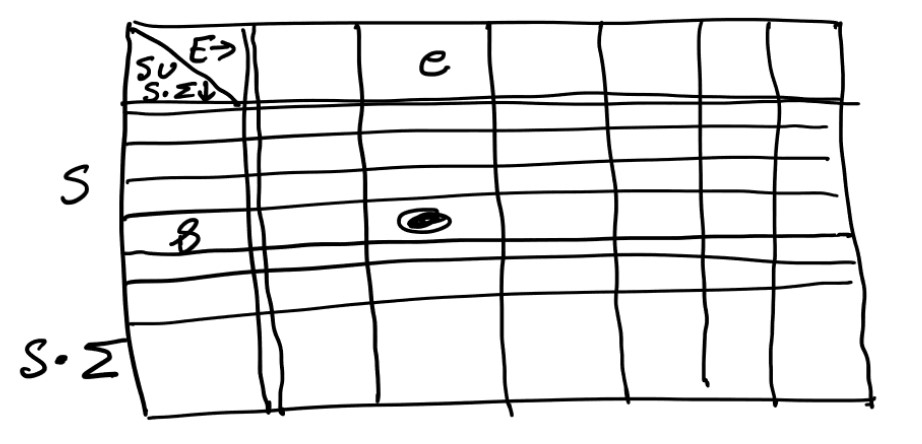
\includegraphics[scale=0.6]{minimally_adequate_teacher.jpg}
\end{center}
\begin{itemize}
    \item $S$: best guess of the states.
    \item $\delta \cdot \Sigma$: All the ``next" states.
    \item $E$: what experiments should I do to tell the states apart.
    
    The entry indexed by $s$ and $e$ is 1 if $se \in L$ and 0 if $se \notin L$, where $L$ is the language we are trying to learn.
    \[T(s,e) = \begin{cases}
    1 & \text{if } se \in L\\
    0& \text{if } se \notin L
    \end{cases}\]
\end{itemize}
Initially $S = E = \{\varepsilon\}$.

\bigbreak\noindent From an observation table, we define a DFA:
\begin{itemize}
    \item $q_0 = row(\varepsilon)$.
    \item $Q = \{row(s) | s \in S\}$.
    \item $F = \{row(s)| s \in S\ \&\ T(s\varepsilon) = T(s) = 1\}$.
    \item $\delta(row(s),x) = row(sx)$ where $x \in \Sigma$.
\end{itemize}
An observation table is \textit{closed} if $\forall t \in S \cdot \Sigma$ $\exists s \in S$ s.t. $row(t) = row(s)$. The states to which I go are in the machine.
\bigbreak\noindent
An observation table is \textit{consistent} if, whenever $s_1,s_2 \in S$,
\[row(s_1) = row(s_2) \Rightarrow \forall x \in \Sigma,\ row(s_1x) = row(s_2x)\]
0's and 1's are arranged the same.
\bigbreak\noindent
This algorithm is called $L^*$ (SEE CLASS EXAMPLES FOR CLOSED AND CONSISTENT TABLE).
\end{document}
